\chapter{Architecture Overview}

\section{Design Overview}

Figure \ref{archi:overview} shows an overview of the architectural design of \lcs. All the components and services are described in detail in the following sections.

\begin{figure}
	\centering
	\centerline{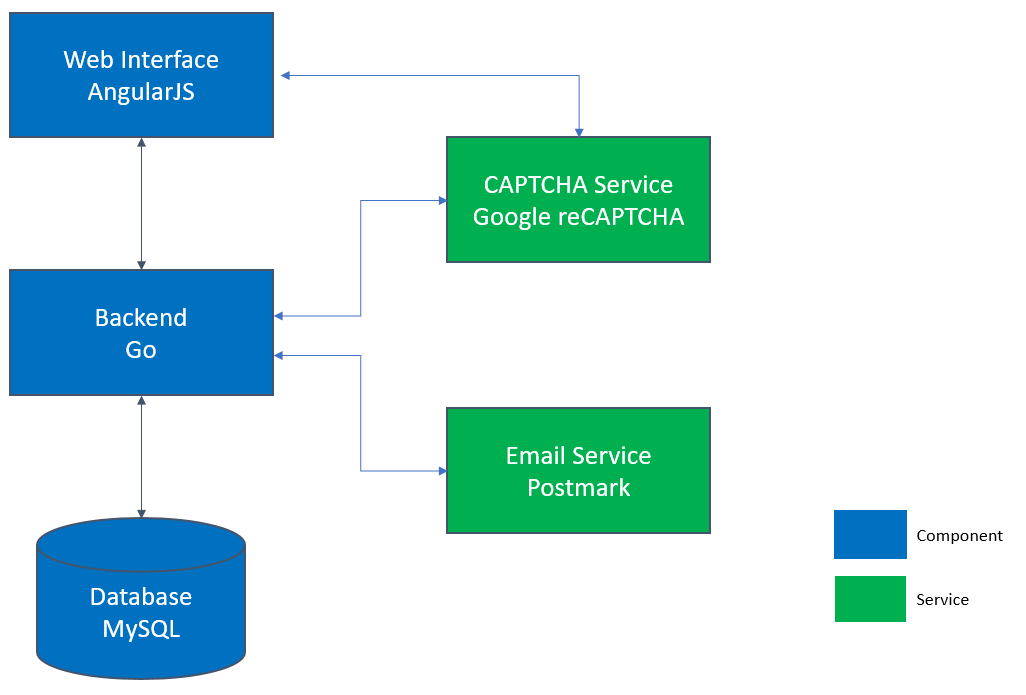
\includegraphics[width=\linewidth]{architecture_overview_new.png}}
	\captionof{figure}{Schematic overview of \lcs architecture, showing its components and the services it uses}
	\label{archi:overview}
\end{figure}

\section{Components}
In the following sections, component denotes a part that directly belongs to the \lcs architecture.

\subsection{Database}

\lcs uses a MySQL database as storage system. MySQL is one of the most widely used relational database management systems. In this project a free to use, open-source version is used. It stores basic entities such as users, their corresponding accounts, ASes deployed by users and connection requests sent between ASes. If a user makes use of a virtual machine to run SCION, configurations for this set up are stored as well. Another purpose is to keep track of the state aforementioned entities are in. It directly interfaces with the back end web server which is the only component it receives queries from.

\subsection{Back End Server}

The centre piece of the \lcs is the back end server. It interfaces with all the other components via a set of well defined APIs, therefore functioning as a mediator. It provides the following functionality:

\begin{itemize}
	\item Serving web pages to the \lcs web interface
	\item Processing of API calls received from the \lcs web interface
	\item Processing of API calls received from SCION \lmi
	\item Controlling access to resources
	\item Preparing emails and handing them over to Postmark servers for sending
	\item Processing and manipulating data retrieved from the database
\end{itemize}

\subsection{Web Interface}

The web interface is the front end part of the \lcs. It is the graphical interface between users and the system. It closely interacts with the back end server, to which it makes API calls and from which it receives all required data. The following functionality is offered by this component:

 \begin{itemize}
 	\item Ability to register new users
 	\item Login for existing users
 	\item A personal page per user showing account details and allowing to download a SCIONLab VM image
 	\item An administrator panel for managing pending user registrations
 	\item A landing page for users, successfully verifying their email address

 \end{itemize}

\section{Services}

\lcs makes use of multiple services to outsource certain tasks. These services are described in the subsections that follow.

\subsection{Postmark}
\label{archi:postmark}

\lcs uses \fnurl{Postmark}{https://postmarkapp.com/} for email sending. An early requirement was to use a local \fnote{MTA}{Mail Transfer Agent - The software running on an email server}. However, as outlined in Section \ref{impl_email_package}, this proved to be very unreliable. The decision was then to switch to an external provider that handles the complexity. Postmark guarantees fast and reliable delivery of all transactional emails sent by \lcs. \cite{postmark}

\subsection{Google reCAPTCHA}
As a measurement against bots that create fake SCIONLab accounts the web interface of \lcs contains a \fnote{CAPTCHA}{Completely Automated Public Turing test to tell Computers and Humans Apart} widget which needs to be solved in order to create an account. \lcs makes use of the Google reCAPTCHA service for implementing this functionality.

\section{Continuous Integration}
\label{archi:ci}

\fnurl{CircleCI}{https://circleci.com/} is a continuous integration utility that, once set up for a project, automatically runs unit tests for newly added code using cloud technologies. The feedback produced includes a comprehensive list of all tests it ran, showing which tests failed and for what reasons. This enables the \lcs development team to validate pull requests before they are merged into the master branch. CircleCI tightly ties into \fnurl{GitHub}{https://github.com/}, showing the outcome of the test suite directly on the pull request page.

 Additionally, new code is reviewed using \fnurl{Reviewable}{https://reviewable.io}. Reviewable keeps track of changes, as pull requests evolve with new commits. To be merged, all tests on CircleCI must pass and all discussions on Reviewable must be resolved.


\section{Deployment}
\label{archi:ansi}

Manually setting up a \lcs instance on a remote machine requires many steps. Hence, doing it often  and for multiple machines very quickly becomes a cumbersome task. To automate this process we use \fnurl{Ansible}{https://www.ansible.com/}. Ansible is an agentless IT automation engine with the goal to end repetitive tasks. It modifies a system in such a way that it matches the state described in configuration files, the playbooks. This makes the deployment, if the playbook is written carefully, idempotent.












